\documentclass{exercise}

\usepackage{makecell}
\usepackage{pgf-pie}

\institute{Institut für Statistik und Wirtschaftsmathematik}
\title{Golbalübung 1}
\author{Joshua Feld, 406718}
\course{Statistik}
\professor{Cramer}
\semester{Sommersemester 2022}
\program{CES (Bachelor)}

\begin{document}
    \maketitle


    \section*{Aufgabe 1}

    \begin{problem}
        Die von einer Bäckerei angebotenen Brotsorten unterscheiden sich u.a. in den Ausprägungen folgender Merkmale:
        \begin{quote}
            Preis pro Stück, Backtemperatur, Zuckerzusatz (ja/nein), Haltbarkeit, Produktionszahl pro Tag, Name, interne Produktnummer.
        \end{quote}
        Geben Sie für jedes Merkmal mögliche Ausprägungen an und ordnen Sie es jeweils den folgenden Merkmalstypen zu:
        \begin{quote}
            qualitativ/nominal, qualitativ/ordinal, quantitativ/diskret, quantitativ/stetig.
        \end{quote}
        Geben Sie darüber hinaus weiter an, welche der Merkmale (speziell) dichotom und welche (speziell) verhältnisskaliert sind.
    \end{problem}

    \subsection*{Lösung}
    \begin{center}
        \begin{tabular}{lcc}
            \toprule
            Merkmal & Merkmalstyp & Mögiche Ausprägungen\\
            \midrule
            Preis pro Stück & \makecell{quantitativ/diskret\\(verhältnisskaliert)} & 2 Euro, 400 Cent, etc.\\
            Backtemperatur & quantitativ/stetig & \(250^\circ\) Celsius, \(392^\circ\) Fahrenheit, etc.\\
            Zuckerzusatz & \makecell{qualitativ/nominal\\(dichotom)} & \makecell{ja, nein\\\(1\), \(0\) (bei entsprechender Codierung)}\\
            Haltbarkeit & \makecell{quantitativ/diskret\\(verhältnisskaliert)} & zwei Tage, drei Monate, etc.\\
            Produktionszahl pro Tag & \makecell{quantitativ/diskret\\(verhältnisskaliert)} & 30 Stück, 100 Stück, etc.\\
            Name & qualitativ/nominal & Vollkornbrot, Sonnenblumenkernbrot, etc.\\
            Interne Produktnummer & qualitativ/nominal & 126, 56, etc.\\
            \bottomrule
        \end{tabular}
    \end{center}


    \section*{Aufgabe 2}

    \begin{problem}
        Bei einer Umfrage in einem Verein werden fünfzig Mitglieder zu ihren Familienstand befragt.
        Die verschiedenen Antwortmöglichkeiten hierbei sind \emph{ledig (\(l\))}, \emph{verheiratet (\(vh\))}, \emph{geschieden (\(g\))} sowie \emph{verwitwet (\(vw\))}.
        Die Umfrage ergibt die folgenden Antworten:
        \[
            vh,\,g,\,l,\,g,\,vw,\,vh,\,vh,\,l,\,vw,\,g,\,g,\,l,\,vh,
        \]
        \[
            g,\,l,\,g,\,l,\,vh,\,vh,\,vh,\,vh,\,l,\,vw,\,g,\,vh,\,g,
        \]
        \[
            vh,\,g,\,vh,\,vh,\,l,\,vw,\,vw,\,vh,\,l,\,vw,\,g,\,vh,\,g,
        \]
        \[
            vh,\,g,\,vh,\,g,\,vw,\,vh,\,vw,\,vh,\,g,\,vh,\,vh.
        \]
        \begin{enumerate}
            \item Bestimmen Sie die absoluten und relativen Häufigkeiten der einzelnen Ausprägungen des Merkmals Familienstand.
            \item Stellen Sie die in a) berechneten absoluten Häufigkeiten in einem Stabdiagramm dar.
            \item Stellen Sie die in a) berechneten relativen Häufigkeiten in einem Kreisdiagramm dar.
        \end{enumerate}
    \end{problem}
    
    \subsection*{Lösung}
    \begin{enumerate}
        \item Auszählen der Umfrage ergibt die folgenden absoluten bzw. relativen Häufigkeiten:
        \begin{center}
            \begin{tabular}{ccc}
                \toprule
                Ausprägung & Absolute Häufigkeit & Relative Häufigkeit\\
                \midrule
                \emph{ledig (\(l\))} & \(8\) & \(\frac{8}{50} = 0,16\)\\
                \emph{verheiratet (\(vh\))} & \(20\) & \(\frac{20}{50} = 0,4\)\\
                \emph{geschieden (\(g\))} & \(14\) & \(\frac{14}{50} = 0,28\)\\
                \emph{verwitwet (\(vw\))} & \(8\) & \(\frac{8}{50} = 0,16\)\\
                \midrule
                Summe & \(n = 50\) & \(1\)\\
                \bottomrule
            \end{tabular}
        \end{center}
        \item\,
        \begin{center}
            \begin{tikzpicture}
                \draw (0,0) -- (8,0);
                \draw[->] (0,0) -- (0,5.5);
                \draw (1,.1) -- (1,-.1) node[below] {ledig};
                \draw (3,.1) -- (3,-.1) node[below] {verheiratet};
                \draw (5,.1) -- (5,-.1) node[below] {geschieden};
                \draw (7,.1) -- (7,-.1) node[below] {verwitwet};
                \draw (.1,0) -- (-.1,0) node[left] {\(0\)};
                \draw (.1,.5) -- (-.1,.5) node[left] {\(2\)};
                \draw (.1,1) -- (-.1,1) node[left] {\(4\)};
                \draw (.1,1.5) -- (-.1,1.5) node[left] {\(6\)};
                \draw (.1,2) -- (-.1,2) node[left] {\(8\)};
                \draw (.1,2.5) -- (-.1,2.5) node[left] {\(10\)};
                \draw (.1,3) -- (-.1,3) node[left] {\(12\)};
                \draw (.1,3.5) -- (-.1,3.5) node[left] {\(14\)};
                \draw (.1,4) -- (-.1,4) node[left] {\(16\)};
                \draw (.1,4.5) -- (-.1,4.5) node[left] {\(18\)};
                \draw (.1,5) -- (-.1,5) node[left] {\(20\)};
                \draw (1,0) -- (1,2);
                \draw[fill=black] (1,2) circle (.075cm);
                \draw (3,0) -- (3,5);
                \draw[fill=black] (3,5) circle (.075cm);
                \draw (5,0) -- (5,3.5);
                \draw[fill=black] (5,3.5) circle (.075cm);
                \draw (7,0) -- (7,2);
                \draw[fill=black] (7,2) circle (.075cm);
            \end{tikzpicture}
        \end{center}
        \item Es bezeichnen \(n_1, \ldots, n_4\) die absoluten Häufigkeiten, \(f_1, \ldots, f_4\) die relativen Häufigkeiten sowie \(\varphi_1, \ldots, \varphi_4\) die Winkel der vier Sektoren zu den Familienständen \(l, vh, g, vw\).
        Dann gilt gemäß Vorlesung mit \(n = 50\):
        \[
            \varphi_j = f_j \cdot 360^\circ = \frac{n_j}{n} \cdot 360^\circ\text{ für }j \in \braces*{1, \ldots, 4}.
        \]
        Hiermit ergibt sich folgende -- gegenüber a) erweiterte -- Tabelle:
        \begin{center}
            \begin{tabular}{cccc}
                \toprule
                Ausprägung & Absolute Häufigkeit & Relative Häufigkeit & Sektor-Winkel\\
                \midrule
                \emph{ledig (\(l\))} & \(8\) & \(\frac{8}{50} = 0,16\) & \(\varphi_1 = 57,6^\circ\)\\
                \emph{verheiratet (\(vh\))} & \(20\) & \(\frac{20}{50} = 0,4\) & \(\varphi_2 = 144^\circ\)\\
                \emph{geschieden (\(g\))} & \(14\) & \(\frac{14}{50} = 0,28\) & \(\varphi_3 = 100,8^\circ\)\\
                \emph{verwitwet (\(vw\))} & \(8\) & \(\frac{8}{50} = 0,16\) & \(\varphi_4 = 57,6^\circ\)\\
                \midrule
                Summe & \(n = 50\) & \(1\) & \(360^\circ\)\\
                \bottomrule
            \end{tabular}
        \end{center}
        \begin{center}
            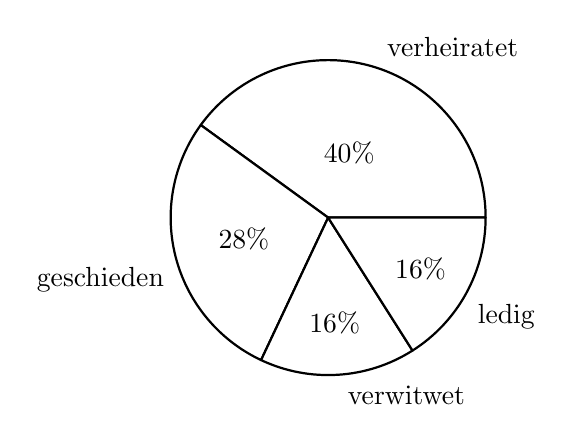
\begin{tikzpicture}
                \pie[radius=2,color={white,white,white,white}] {40/verheiratet,28/geschieden,16/verwitwet,16/ledig};
            \end{tikzpicture}
        \end{center}
    \end{enumerate}


    \section*{Aufgabe 3}

    \begin{problem}
        Im Folgenden Kreisdiagramm ist die Häufigkeitsverteilung der gültigen Zweitstimmen bei der Bundestagswahl 2005 dargestellt:
        \begin{center}
            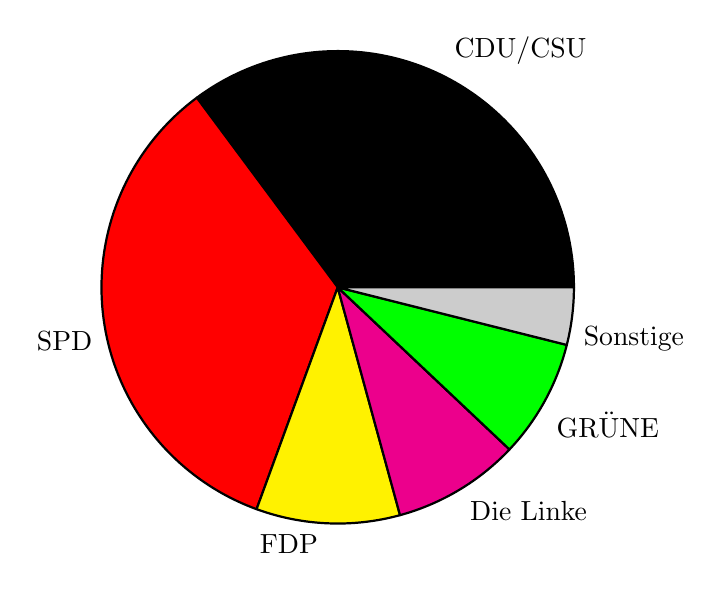
\begin{tikzpicture}
                \pie[hide number,radius=3,color={black,red,yellow,magenta,green,white!80!black}] {35.17/{CDU/CSU},34.25/SPD,9.83/FDP,8.71/Die Linke,8.12/GRÜNE, 3.92/Sonstige};
            \end{tikzpicture}
        \end{center}
        Messen Sie die Winkel der dargestellten Kreissektoren und berechnen Sie hieraus (näherungsweise) die prozentualen Stimmenanteile der einzelnen Parteien.
    \end{problem}
    
    \subsection*{Lösung}
    Es bezeichnen \(\varphi_1, \ldots, \varphi_6\) die Sektorenwinkel zu CDU/CSU, \(\ldots\), Sonstige (in dieser Reihenfolge).
    Dann sollten die Winkel zunächst möglichst genau gemessen werden.
    (Hierzu Strahlen, die die Sektoren begrenzen geeignet verlängern.)
    Man erhält (näherungsweise) folgende Winkel:
    \begin{center}
        \begin{tabular}{lc}
            \toprule
            Partei & Sektorwinkel\\
            \midrule
            CDU/CSU & \(\varphi_1 \approx 126,5^\circ\)\\
            SPD & \(\varphi_2 \approx 123,5^\circ\)\\
            FDP & \(\varphi_3 \approx 35^\circ\)\\
            Die Linke & \(\varphi_4 \approx 31,5^\circ\)\\
            GRÜNE & \(\varphi_5 \approx 29,4^\circ\)\\
            Sonstige & \(\varphi_6 \approx 14,1^\circ\)\\
            \midrule
            Summe & \(360^\circ\)\\
            \bottomrule
        \end{tabular}
    \end{center}
    Es bezeichnen \(f_1, \ldots, f_6\) die zugehörigen relativen Häufigkeiten.
    Dann gilt gemäß Vorlesung (vgl. Aufgabe 2, c)):
    \[
        \varphi_j = f_j \cdot 360^\circ \iff f_j = \frac{\varphi_j}{360^\circ}\text{ für }j \in \braces*{1, \ldots, 6}.
    \]
    Einsetzen der gemessenen Winkel ergibt die folgende erweiterte Tabelle.
    \begin{center}
        \begin{tabular}{lccc}
            \toprule
            Partei & Sektorwinkel & Relative Häufigkeit & prozentualer Stimmenanteil\\
            \midrule
            CDU/CSU & \(\varphi_1 \approx 126,5^\circ\) & \(f_1 \approx 0,3514\) & \(35,14\%\)\\
            SPD & \(\varphi_2 \approx 123,5^\circ\) & \(f_2 \approx 0,3431\) & \(34,31\%\)\\
            FDP & \(\varphi_3 \approx 35^\circ\) & \(f_3 \approx 0,0972\) & \(9,72\%\)\\
            Die Linke & \(\varphi_4 \approx 31,5^\circ\) & \(f_4 \approx 0,0875\) & \(8,75\%\)\\
            GRÜNE & \(\varphi_5 \approx 29,4^\circ\) & \(f_5 \approx 0,0817\) & \(8,17\%\)\\
            Sonstige & \(\varphi_6 \approx 14,1^\circ\) & \(f_6 \approx 0,0392\) & \(3,92\%\)\\
            \midrule
            Summe & \(360^\circ\) & \(1,0001\) & \(100,01\%\)\\
            \bottomrule
        \end{tabular}
    \end{center}


    \section*{Aufgabe 4}

    \begin{problem}
        Bei einem Quiz mussten die fünfzehn Teilnehmer(innen) jeweils acht Fragen beantworten.
        Hierbei ergaben sich für die einzelnen Personen die folgenden Anzahlen richtiger Antworten:
        \[
            x_1 = 3, x_2 = 5, x_3 = 5, x_4 = 7, x_5 = 4, x_6 = 8, x_7 = 2, x_8 = 4,
        \]
        \[
            x_9 = 4, x_{10} = 6, x_{11} = 2, x_{12} = 7, x_{13} = 6, x_{14} = 4, x_{15} = 6.
        \]
        \begin{enumerate}
            \item Bestimmen Sie die zugehörige Rangwertreihe sowie die Ränge der einzelnen Beobachtungswerte \(x_1, \ldots, x_{15}\).
            \item Berechnen Sie zu dem gegebenen Datensatz \(x_1, \ldots, x_{15}\) die absoluten und relativen Häufigkeiten der \emph{verschiedenen} Beobachtungswerte, und bestimmen Sie die zugehörigen Modalwerte (d.h. die Ausprägungen mit maximaler (relativer) Häufigkeit unter den verschiedenen Beobachtungswerten).
        \end{enumerate}
    \end{problem}

    \subsection*{Lösung}
    \begin{enumerate}
        \item Die zugehörige Rangwertreihe \(x_{\parentheses*{1}} \le \cdots \le x_{\parentheses*{15}}\) ergibt sich durch aufsteigende Anordnung der gegebenen Beobachtungen \(x_1, \ldots, x_15\):
        \[
            x_{\parentheses*{1}} = 2, x_{\parentheses*{2}} = 2, x_{\parentheses*{3}} = 3, x_{\parentheses*{4}} = 4, x_{\parentheses*{5}} = 4, x_{\parentheses*{6}} = 4, x_{\parentheses*{7}} = 4, x_{\parentheses*{8}} = 5,
        \]
        \[
            x_{\parentheses*{9}} = 5, x_{\parentheses*{10}} = 6, x_{\parentheses*{11}} = 6, x_{\parentheses*{12}} = 6, x_{\parentheses*{13}} = 7, x_{\parentheses*{14}} = 7, x_{\parentheses*{15}} = 8.
        \]
        Die Rangwertreihe zeigt:
        \begin{itemize}
            \item Nur \(3\) und \(8\) kommen jeweils einmal vor.
            \item Die übrigen Beobachtungswerte kommen jedoch jeweils mehrfach vor. 
        \end{itemize}
        Für diese \(i \in \braces*{1, \ldots, 15}\) wird der Rang \(R\parentheses*{x_i}\) gemäß Vorlesung als das arithmetische Mittel der betreffenden Positionen berechnet.
        Beispiele:
        \begin{align*}
            R\parentheses*{x_2} &= R\parentheses*{5} = \frac{8 + 9}{2} = \frac{17}{2} = 8,5,\\
            R\parentheses*{x_5} &= R\parentheses*{4} = \frac{4 + 5 + 6 + 7}{4} = \frac{22}{4} = 5,5.
        \end{align*}
        Auf diese Weise erhält man die folgenden Ränge zu \(x_1, \ldots, x_{15}\):
        \begin{center}
            \begin{tabular}{lccccccccccccccc}
                \toprule
                \(i\) & \(1\) & \(2\) & \(3\) & \(4\) & \(5\) & \(6\) & \(7\) & \(8\) & \(9\) & \(10\) & \(11\) & \(12\) & \(13\) & \(14\) & \(15\)\\
                \(x_i\) & \(3\) & \(5\) & \(5\) & \(7\) & \(4\) & \(8\) & \(2\) & \(4\) & \(4\) & \(6\) & \(2\) & \(7\) & \(6\) & \(4\) & \(6\)\\
                \midrule
                \(R\parentheses*{x_i}\) & \(3\) & \(8,5\) & \(8,5\) & \(13,5\) & \(5,5\) & \(15\) & \(1,5\) & \(5,5\) & \(5,5\) & \(11\) & \(1,5\) & \(13,5\) & \(11\) & \(5,5\) & \(11\)\\
                \bottomrule
            \end{tabular}
        \end{center}
        \item Der Rangwertreihe aus a) entnimmt man, dass unter \(x_1, \ldots, x_{15}\) die sieben verschiedenen Werte \(2, \ldots, 8\) vorkommen.
        Diese -- aufsteigend angeordneten -- Werte seien (analog zur Vorlesung) mit \(u_{\parentheses*{1}}, \ldots, u_{\parentheses*{7}}\) bezeichnet.

        Die absoluten Häufigkeiten \(n_{\parentheses*{1}}, \ldots, n_{\parentheses*{7}}\) von \(u_{\parentheses*{1}}, \ldots, u_{\parentheses*{7}}\) kann man ebenfalls unmittelbar aus der Rangwertreihe ablesen und hieraus die relativen Häufigkeiten gemäß
        \[
            f_{\parentheses*{j}} = \frac{n_{\parentheses*{j}}}{n}, \quad j \in \braces*{1, \ldots, 7},
        \]
        mit \(n = 15\) berechnen.
        \begin{center}
            \begin{tabular}{lccccccccc}
                \toprule
                & \(j\) & \(1\) & \(2\) & \(3\) & \(4\) & \(5\) & \(6\) & \(7\) & Summe\\
                \midrule
                Beobachtungswert & \(u_{\parentheses*{j}}\) & \(2\) & \(3\) & \(4\) & \(5\) & \(6\) & \(7\) & \(8\) &\\
                Absolute Häufigkeit & \(n_{\parentheses*{j}}\) & \(2\) & \(1\) & \(4\) & \(2\) & \(3\) & \(2\) & \(1\) & \(15\)\\
                Relative Häufigkeit & \(f_{\parentheses*{j}}\) & \(\frac{2}{15}\) & \(\frac{1}{15}\) & \(\frac{4}{15}\) & \(\frac{2}{15}\) & \(\frac{3}{15}\) & \(\frac{2}{15}\) & \(\frac{1}{15}\) & \(1\)\\
                \bottomrule
            \end{tabular}
        \end{center}
        Der Häufigkeitstabelle entnimmt man:
        \[
            \max\braces*{f_{\parentheses*{j}} : j \in \braces*{1, \ldots, 7}} = \frac{4}{15} = f_{\parentheses*{3}} > f_{\parentheses*{j}}\text{ für alle }j \ne 3.
        \]
        Damit ist \(u_{\parentheses*{3}} = 4\) der eizige Modalwert.
    \end{enumerate}
\end{document}
